\documentclass{article}
\usepackage{tikz}
\usetikzlibrary{patterns, shapes.geometric}
\usepackage{amsmath}

\author{Cser Máté}

\begin{document}

\begin{tikzpicture}
    \draw (0,0) -- (2,0) -- (2,2) -- (1,3) -- (0,2) -- cycle;
    \draw (0,2) -- (2,2);
    \draw (0,0) -- (0,2);

    \begin{scope}[scale=2]
        \draw (4,0) -- (6,0) -- (6,2) -- (5,3) -- (4,2) -- cycle;
        \draw (4,2) -- (6,2);
        \draw (4,0) -- (4,2);
    \end{scope}
\end{tikzpicture}

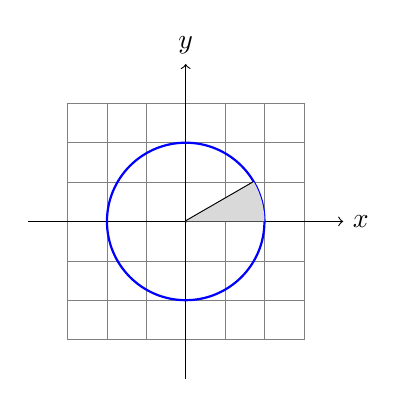
\begin{tikzpicture}
    \draw[step=0.5,gray,very thin] (-1.5,-1.5) grid (1.5,1.5);
    \draw[->] (-2,0) -- (2,0) node[right] {$x$};
    \draw[->] (0,-2) -- (0,2) node[above] {$y$};
    \draw[thick,blue] (0,0) circle(1);
    \draw[thick] (0,0) -- (cos 30,sin 30);
    \fill[gray!30] (0,0) -- (1,0) arc[start angle=0, end angle=30, radius=1] -- cycle;
\end{tikzpicture}

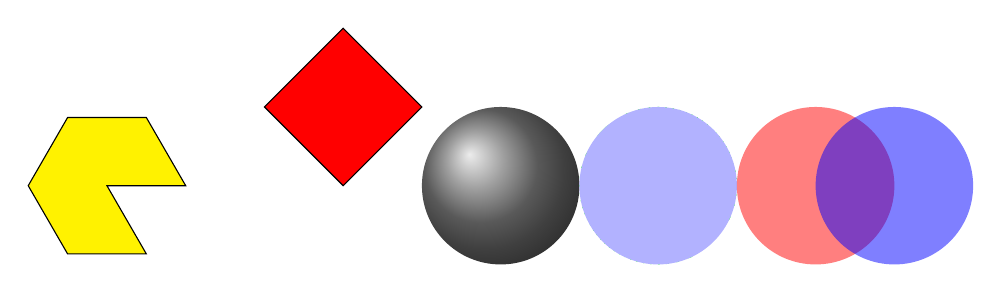
\begin{tikzpicture}
    \draw[fill=yellow] (0,0) \foreach \x in {0,60,...,300} { -- (\x:1cm)} -- cycle;
    \draw[fill=red] (3,0) -- (4,1) -- (3,2) -- (2,1) -- cycle;
    \shade[ball color=gray] (5,0) circle(1);
    \fill[pattern=north east lines, pattern color=green] (7,0) circle(1);
    \fill[blue!30] (7,0) circle(1);
    \fill[red,opacity=0.5] (9,0) circle(1);
    \fill[blue,opacity=0.5] (10,0) circle(1);
\end{tikzpicture}

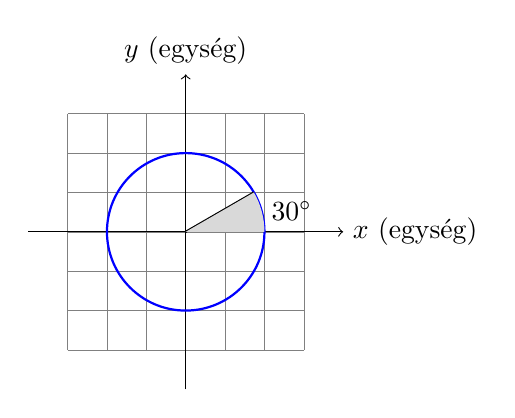
\begin{tikzpicture}
    \draw[step=0.5,gray,very thin] (-1.5,-1.5) grid (1.5,1.5);
    \draw[->] (-2,0) -- (2,0) node[right] {$x$ (egység)};
    \draw[->] (0,-2) -- (0,2) node[above] {$y$ (egység)};
    \draw[thick,blue] (0,0) circle(1);
    \draw[thick] (0,0) -- (cos 30,sin 30);
    \node at (cos 15,sin 15) [right] {$30^\circ$};
    \fill[gray!30] (0,0) -- (1,0) arc[start angle=0, end angle=30, radius=1] -- cycle;
\end{tikzpicture}

\begin{tikzpicture}[node distance=2cm]
    \node (start) [draw, rectangle] {Start};
    \node (process) [draw, rectangle, below of=start] {Feldolgozás};
    \node (decision) [draw, diamond, aspect=2, below of=process] {Döntés};
    \node (end) [draw, rectangle, below of=decision] {Vége};
    
    \draw[->] (start) -- (process);
    \draw[->] (process) -- (decision);
    \draw[->] (decision) -- (end);
    \draw[->] (decision.east) -- ++(2,0) node[right] {Igen};
    \draw[->] (decision.west) -- ++(-2,0) node[left] {Nem};
\end{tikzpicture}

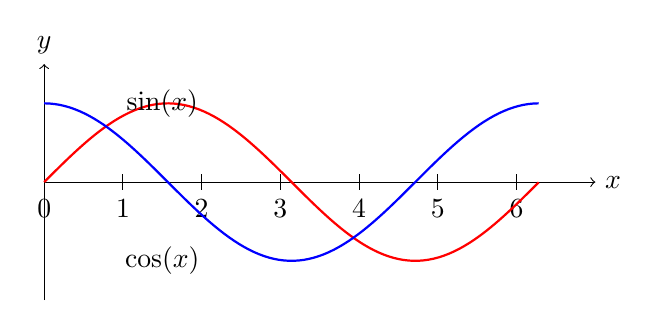
\begin{tikzpicture}
    \draw[->] (0,-1.5) -- (0,1.5) node[above] {$y$};
    \draw[->] (0,0) -- (7,0) node[right] {$x$};
    \foreach \x in {0,1,...,6}
        \draw (\x,0.1) -- (\x,-0.1) node[below] {$\x$};
    \draw[red,thick] plot[domain=0:6.28,samples=100] (\x,{sin(\x r)});
    \node at (1.5,1) {$\sin(x)$};
    \draw[blue,thick] plot[domain=0:6.28,samples=100] (\x,{cos(\x r)});
    \node at (1.5,-1) {$\cos(x)$};
\end{tikzpicture}

\end{document}
